\documentclass[11pt]{article}
\usepackage{amsmath, amssymb, physics, mathtools, bm}
\usepackage{tikz, pgfplots}
\pgfplotsset{compat=1.18}
\usepackage[margin=2.3cm]{geometry}
\usepackage{siunitx, booktabs, hyperref}
\usepackage{braket}

\newcommand{\D}{\mathrm{D}}
\newcommand{\de}{\mathrm{d}}
\newcommand{\pd}[2]{\frac{\partial #1}{\partial #2}}
\newcommand{\pdd}[2]{\frac{\partial^{2} #1}{\partial #2^{2}}}
\newcommand{\Lap}{\nabla^{2}}

\title{B1 Flows, Fluctuations and Complexity --- Model Solutions, 2017}
\author{}
\date{}

\begin{document}
\maketitle

%==============================================================
\section*{Question 1 --- Surface gravity--capillary waves}

\textbf{Problem.} Derive Laplace's equation for the velocity potential of an incompressible irrotational flow. For deep-water linear surface waves with $\eta=A\sin(kx-\omega t)$ find $\phi$, the dispersion relation, the particle paths, and (with surface tension) $\omega^{2}=c_{1}k+c_{2}k^{3}$.

\subsection*{Laplace's equation}

Irrotational $\curl{\vb u}=0$ implies potential exists:
\[ \vb u=\grad\phi. \]
Take divergence:
\[ \div{\vb u}=\div(\grad\phi)=\Lap\phi. \]
Apply incompressibility $\div{\vb u}=0$:
\[ \boxed{\;\Lap\phi=0.\;} \]

\subsection*{Boundary conditions}

\textbf{Kinematic (}$\partial_t\eta=\partial_z\phi$ at $z=0$\textbf{)}: a fluid particle on the surface stays on the surface, so the vertical fluid velocity equals the surface vertical velocity (linearised: evaluated at $z=0$).

\textbf{Dynamic (}$\partial_t\phi=-g\eta$ at $z=0$\textbf{)}: linearised Bernoulli at the free surface with $p=p_\text{atm}$ gives $\partial_t\phi+g\eta+p_\text{atm}/\rho=\text{const}$; absorb the constant into $\phi$.

\textbf{Depth condition}: fluid at rest as $z\to-\infty$:
\[ \grad\phi\to 0,\qquad \pd{\phi}{z}\to 0\quad(z\to-\infty). \]

\subsection*{Velocity potential and dispersion relation}

Try separable form $\pi/2$ out of phase with $\eta$:
\[ \phi(x,z,t)=f(z)\cos(kx-\omega t). \]
Compute $\partial_x^{2}\phi$:
\[ \partial_x^{2}\phi=-k^{2}f(z)\cos(kx-\omega t). \]
Compute $\partial_z^{2}\phi$:
\[ \partial_z^{2}\phi=f''(z)\cos(kx-\omega t). \]
Sum and apply $\Lap\phi=0$:
\[ \bigl(f''(z)-k^{2}f(z)\bigr)\cos(kx-\omega t)=0. \]
Reduce to ODE:
\[ f''(z)-k^{2}f(z)=0. \]
General solution:
\[ f(z)=Ce^{kz}+De^{-kz}. \]
Apply $z\to-\infty$ decay (with $k>0$, $e^{-kz}\to\infty$):
\[ D=0. \]
Hence:
\[ \phi=Ce^{kz}\cos(kx-\omega t). \]
Compute $\partial_t\eta$ and $\partial_z\phi|_{z=0}$:
\[ \partial_t\eta=-A\omega\cos(kx-\omega t),\qquad \partial_z\phi|_0=Ck\cos(kx-\omega t). \]
Equate (kinematic BC):
\[ -A\omega\cos(kx-\omega t)=Ck\cos(kx-\omega t). \]
Solve for $C$:
\[ C=-\frac{A\omega}{k}. \]
Velocity potential:
\begin{equation}
\boxed{\;\phi(x,z,t)=-\frac{A\omega}{k}\,e^{kz}\cos(kx-\omega t).\;}
\label{eq:phi-deep}
\end{equation}
Compute $\partial_t\phi$ at $z=0$:
\[ \partial_t\phi|_0=-\frac{A\omega^{2}}{k}\sin(kx-\omega t). \]
Apply dynamic BC $\partial_t\phi=-g\eta$:
\[ -\frac{A\omega^{2}}{k}\sin(kx-\omega t)=-gA\sin(kx-\omega t). \]
Cancel $-A\sin(kx-\omega t)$:
\[ \frac{\omega^{2}}{k}=g. \]
Multiply by $k$:
\begin{equation}
\boxed{\;\omega^{2}=gk.\;}
\label{eq:disp-deep}
\end{equation}

\subsection*{Particle paths}

Lagrangian displacement $(\xi,\zeta)$ of a particle about $(x_0,z_0)$:
\[ \dot\xi=u=\partial_x\phi,\qquad \dot\zeta=w=\partial_z\phi. \]
Differentiate $\phi=-(A\omega/k)e^{kz}\cos(kx-\omega t)$ w.r.t.\ $x$:
\[ \partial_x\phi=-\frac{A\omega}{k}\,e^{kz}\cdot(-k)\sin(kx-\omega t). \]
Simplify:
\[ \partial_x\phi=A\omega\,e^{kz}\sin(kx-\omega t). \]
Differentiate w.r.t.\ $z$:
\[ \partial_z\phi=-A\omega\,e^{kz}\cos(kx-\omega t). \]
Evaluate at the mean position $(x_0,z_0)$ (linear theory):
\[ u=A\omega\,e^{kz_0}\sin(kx_0-\omega t),\qquad w=-A\omega\,e^{kz_0}\cos(kx_0-\omega t). \]
Integrate $u$ in time:
\[ \xi=\int A\omega\,e^{kz_0}\sin(kx_0-\omega t)\,\de t. \]
Use $\int\sin(kx_0-\omega t)\,\de t=\tfrac{1}{\omega}\cos(kx_0-\omega t)$:
\[ \xi=A\,e^{kz_0}\cos(kx_0-\omega t). \]
Integrate $w$ in time:
\[ \zeta=\int -A\omega\,e^{kz_0}\cos(kx_0-\omega t)\,\de t. \]
Use $\int\cos(kx_0-\omega t)\,\de t=-\tfrac{1}{\omega}\sin(kx_0-\omega t)$:
\[ \zeta=A\,e^{kz_0}\sin(kx_0-\omega t). \]
Square and add (apply $\sin^{2}+\cos^{2}=1$):
\[ \xi^{2}+\zeta^{2}=A^{2}e^{2kz_0}. \]
Circular paths of radius $R(z_0)=A\,e^{kz_0}$, decaying exponentially with depth:
\[ \boxed{\;R(z_0)=A\,e^{kz_0}.\;} \]

\begin{center}
\begin{tikzpicture}[>=stealth, scale=1.0]
  \draw[->] (-0.5,0) -- (6.5,0) node[right] {$x$};
  \draw[->] (0,-3.5) -- (0,1.0) node[above] {$z$};
  \draw[dashed] (0,0) -- (6.2,0);
  \node[left] at (0,0) {$0$};
  % Three depth levels with decreasing circles
  \node[circle,fill,inner sep=1.2pt] (P1) at (1.5,-0.3) {};
  \draw (1.5,-0.3) circle (0.5);
  \node[right] at (2.05,-0.3) {$R=A$};
  \node[circle,fill,inner sep=1.2pt] (P2) at (3.5,-1.4) {};
  \draw (3.5,-1.4) circle (0.27);
  \node[right] at (3.8,-1.4) {$R=A\,e^{kz_{0}}$};
  \node[circle,fill,inner sep=1.2pt] (P3) at (5.5,-2.6) {};
  \draw (5.5,-2.6) circle (0.10);
  \node[right] at (5.65,-2.6) {small};
\end{tikzpicture}
\end{center}

\subsection*{Surface tension: dispersion relation}

Modified dynamic BC at $z=0$:
\[ \pd{\phi}{t}=-g\eta+\frac{\sigma}{\rho}\pdd{\eta}{x}. \]
Compute $\partial_x^{2}\eta$:
\[ \pdd{\eta}{x}=-Ak^{2}\sin(kx-\omega t). \]
Insert $\partial_t\phi|_0=-(A\omega^{2}/k)\sin(kx-\omega t)$ and $\eta$:
\[ -\frac{A\omega^{2}}{k}\sin(kx-\omega t)=-gA\sin(kx-\omega t)-\frac{\sigma}{\rho}Ak^{2}\sin(kx-\omega t). \]
Cancel $-A\sin(kx-\omega t)$:
\[ \frac{\omega^{2}}{k}=g+\frac{\sigma k^{2}}{\rho}. \]
Multiply by $k$:
\begin{equation}
\boxed{\;\omega^{2}=gk+\frac{\sigma}{\rho}k^{3},\qquad c_{1}=g,\quad c_{2}=\sigma/\rho.\;}
\label{eq:disp-cap}
\end{equation}
Wave speed $c=\omega/k$:
\[ c^{2}=\frac{\omega^{2}}{k^{2}}=\frac{g}{k}+\frac{\sigma k}{\rho}. \]
Take square root:
\[ c(k)=\sqrt{\frac{g}{k}+\frac{\sigma k}{\rho}}. \]
Minimise $c^{2}$ via $\de(c^{2})/\de k=0$:
\[ -\frac{g}{k^{2}}+\frac{\sigma}{\rho}=0. \]
Solve for $k_{*}$:
\[ k_{*}=\sqrt{g\rho/\sigma}. \]
Insert $k_{*}=\sqrt{g\rho/\sigma}$ into $c^{2}$:
\[ c_{\min}^{2}=\frac{g}{\sqrt{g\rho/\sigma}}+\frac{\sigma}{\rho}\sqrt{g\rho/\sigma}. \]
Simplify first term:
\[ \frac{g}{\sqrt{g\rho/\sigma}}=\sqrt{g\sigma/\rho}. \]
Simplify second term:
\[ \frac{\sigma}{\rho}\sqrt{g\rho/\sigma}=\sqrt{g\sigma/\rho}. \]
Sum:
\[ c_{\min}^{2}=2\sqrt{g\sigma/\rho}. \]
Take square root:
\[ c_{\min}=\bigl(4g\sigma/\rho\bigr)^{1/4}. \]

\begin{center}
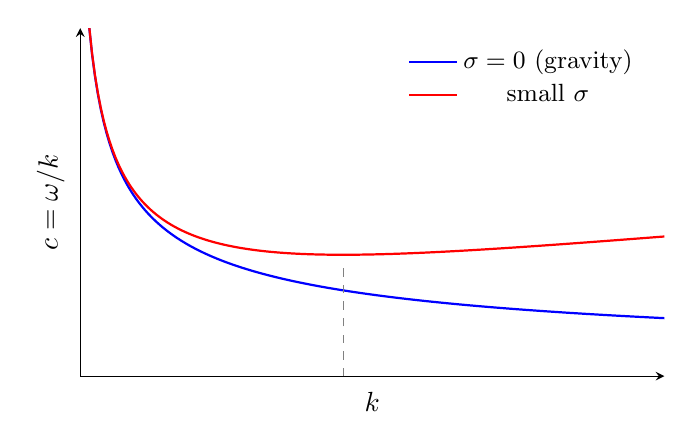
\begin{tikzpicture}[>=stealth, scale=1.0]
  \begin{axis}[
    width=9cm, height=6cm,
    axis lines=left,
    xlabel={$k$}, ylabel={$c=\omega/k$},
    xtick=\empty, ytick=\empty,
    xmin=0.05, xmax=4, ymin=0, ymax=3,
    domain=0.05:4, samples=200,
    legend pos=north east,
    legend style={draw=none, font=\small}
  ]
    \addplot[thick, blue]   {sqrt(1/x)};            \addlegendentry{$\sigma=0$ (gravity)}
    \addplot[thick, red]    {sqrt(1/x + 0.3*x)};   \addlegendentry{small $\sigma$}
    \draw[dashed,gray] (axis cs:1.83,0) -- (axis cs:1.83,0.93);
    \node[below] at (axis cs:1.83,0) {$k_{*}$};
  \end{axis}
\end{tikzpicture}
\end{center}

Short waves ($k\gg k_{*}$, small $\lambda$) most affected: the curvature $\partial_x^{2}\eta\propto k^{2}$ amplifies the surface-tension restoring force, while gravity $g/k$ becomes negligible. Long waves ($k\ll k_*$) are gravity-dominated.

%==============================================================
\section*{Question 2 --- Reynolds number, cylinder with source, Bernoulli, Torricelli}

\textbf{Problem.} Derive Re by non-dimensionalising 2-D steady NS; for $\phi=Ur\cos\theta+\mu\cos\theta/r+m\log r$ around a cylinder of radius $a$ with outward normal velocity $V$, find $\mu,m$; for $V=4U$ locate the upstream stagnation point; derive Bernoulli; find efflux speed and flux from a tank.

\subsection*{Reynolds number}

Steady 2-D incompressible NS (drop gravity / absorb into pressure):
\[ (\vb u\cdot\grad)\vb u=-\frac{1}{\rho}\grad p+\nu\Lap\vb u. \]
Introduce scales $\vb u=U\vb u^{*}$, $\grad=L^{-1}\grad^{*}$, $p=\rho U^{2}p^{*}$:
\[ \frac{U^{2}}{L}(\vb u^{*}\cdot\grad^{*})\vb u^{*}=-\frac{1}{\rho}\cdot\frac{\rho U^{2}}{L}\grad^{*}p^{*}+\frac{\nu U}{L^{2}}\nabla^{*2}\vb u^{*}. \]
Cancel $\rho$ in the pressure term:
\[ \frac{U^{2}}{L}(\vb u^{*}\cdot\grad^{*})\vb u^{*}=-\frac{U^{2}}{L}\grad^{*}p^{*}+\frac{\nu U}{L^{2}}\nabla^{*2}\vb u^{*}. \]
Divide through by $U^{2}/L$:
\[ (\vb u^{*}\cdot\grad^{*})\vb u^{*}=-\grad^{*}p^{*}+\frac{\nu}{UL}\nabla^{*2}\vb u^{*}. \]
Identify dimensionless coefficient $1/\mathrm{Re}$:
\[ (\vb u^{*}\cdot\grad^{*})\vb u^{*}=-\grad^{*}p^{*}+\frac{1}{\mathrm{Re}}\nabla^{*2}\vb u^{*}. \]
Hence:
\[ \boxed{\;\mathrm{Re}=\frac{UL}{\nu}.\;} \]

Behaviour: $\mathrm{Re}\ll 1$ Stokes (creeping) flow, viscosity dominates, time-reversible streamlines. $\mathrm{Re}\sim O(1)$ steady laminar flow with separation possible. $\mathrm{Re}\gtrsim 40$ unsteady wake (von K\'arm\'an street). $\mathrm{Re}\gtrsim 10^{3}$--$10^{5}$ transition to turbulence; inertia dominates, viscous effects confined to thin boundary layers.

\subsection*{Cylinder with source: $\mu$, $m$}

Compute $u_r=\partial\phi/\partial r$:
\[ u_r=\pd{}{r}\!\left[Ur\cos\theta+\frac{\mu\cos\theta}{r}+m\log r\right]. \]
Differentiate term-by-term:
\[ u_r=U\cos\theta-\frac{\mu\cos\theta}{r^{2}}+\frac{m}{r}. \]
Compute $u_\theta=(1/r)\,\partial\phi/\partial\theta$:
\[ u_\theta=\frac{1}{r}\pd{}{\theta}\!\left[Ur\cos\theta+\frac{\mu\cos\theta}{r}+m\log r\right]. \]
Differentiate term-by-term:
\[ u_\theta=\frac{1}{r}\!\left[-Ur\sin\theta-\frac{\mu\sin\theta}{r}\right]=-U\sin\theta-\frac{\mu\sin\theta}{r^{2}}. \]
Apply normal BC $u_r(a,\theta)=V$ for all $\theta$:
\[ U\cos\theta-\frac{\mu\cos\theta}{a^{2}}+\frac{m}{a}=V. \]
Match $\cos\theta$ coefficient:
\[ U-\frac{\mu}{a^{2}}=0. \]
Solve for $\mu$:
\[ \mu=Ua^{2}. \]
Match constant ($\theta$-independent) part:
\[ \frac{m}{a}=V. \]
Solve for $m$:
\[ m=Va. \]
\[ \boxed{\;\mu=Ua^{2},\qquad m=Va.\;} \]
Potential and velocities:
\[ \phi=U\cos\theta\Bigl(r+\frac{a^{2}}{r}\Bigr)+Va\,\log r, \]
\[ u_r=U\cos\theta\Bigl(1-\frac{a^{2}}{r^{2}}\Bigr)+\frac{Va}{r},\qquad u_\theta=-U\sin\theta\Bigl(1+\frac{a^{2}}{r^{2}}\Bigr). \]

\subsection*{Stagnation point for $V=4U$}

By symmetry, the stagnation point lies on $\theta=\pi$ (upstream axis). On this axis $\sin\theta=0$ so $u_\theta\equiv 0$; require $u_r=0$ with $V=4U$:
\[ U\cos\pi\Bigl(1-\frac{a^{2}}{r^{2}}\Bigr)+\frac{4Ua}{r}=0. \]
Substitute $\cos\pi=-1$:
\[ -U\Bigl(1-\frac{a^{2}}{r^{2}}\Bigr)+\frac{4Ua}{r}=0. \]
Cancel $U$:
\[ -\Bigl(1-\frac{a^{2}}{r^{2}}\Bigr)+\frac{4a}{r}=0. \]
Multiply by $r^{2}$:
\[ -r^{2}+a^{2}+4ar=0. \]
Rearrange:
\[ r^{2}-4ar-a^{2}=0. \]
Apply quadratic formula:
\[ r=\frac{4a\pm\sqrt{16a^{2}+4a^{2}}}{2}. \]
Simplify the discriminant:
\[ r=\frac{4a\pm\sqrt{20a^{2}}}{2}=\frac{4a\pm 2a\sqrt{5}}{2}. \]
Divide by $2$:
\[ r=2a\pm a\sqrt{5}=(2\pm\sqrt{5})a. \]
Take the root with $r>a$ (outside cylinder); $(2-\sqrt{5})a<0$ is rejected:
\[ \boxed{\;r_{\text{stag}}=(2+\sqrt{5})\,a.\;} \]

\begin{center}
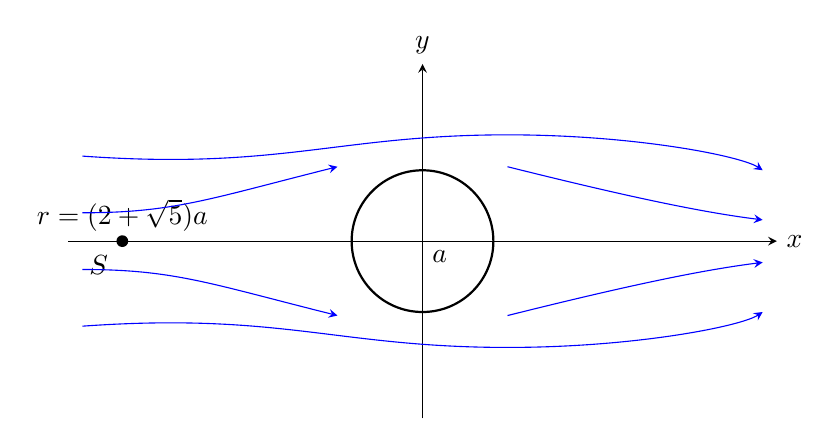
\begin{tikzpicture}[>=stealth, scale=0.9]
  \draw[->] (-5,0) -- (5,0) node[right] {$x$};
  \draw[->] (0,-2.5) -- (0,2.5) node[above] {$y$};
  \draw[thick] (0,0) circle (1);
  \node[below right] at (0,0) {$a$};
  \node[circle,fill,inner sep=1.5pt,label=below left:{$S$}] at (-4.236,0) {};
  \node[above] at (-4.236,0) {$r=(2+\sqrt 5)a$};
  % streamlines (schematic)
  \draw[->,blue] (-4.8,1.2) .. controls (-2,1.0) and (-1.2,1.5) .. (1.2,1.5) .. controls (3,1.5) and (4.5,1.2) .. (4.8,1.0);
  \draw[->,blue] (-4.8,-1.2) .. controls (-2,-1.0) and (-1.2,-1.5) .. (1.2,-1.5) .. controls (3,-1.5) and (4.5,-1.2) .. (4.8,-1.0);
  \draw[->,blue] (-4.8,0.4) .. controls (-3.5,0.4) and (-3,0.6) .. (-1.2,1.05);
  \draw[->,blue] (-4.8,-0.4) .. controls (-3.5,-0.4) and (-3,-0.6) .. (-1.2,-1.05);
  \draw[->,blue] (1.2,1.05) .. controls (3,0.6) and (4,0.4) .. (4.8,0.3);
  \draw[->,blue] (1.2,-1.05) .. controls (3,-0.6) and (4,-0.4) .. (4.8,-0.3);
\end{tikzpicture}
\end{center}

\subsection*{Bernoulli along streamlines}

Steady, inviscid, incompressible Euler with gravity:
\[ (\vb u\cdot\grad)\vb u+\frac{1}{\rho}\grad p+g\hat{\vb k}=0. \]
Write $g\hat{\vb k}=\grad(gz)$:
\[ (\vb u\cdot\grad)\vb u+\frac{1}{\rho}\grad p+\grad(gz)=0. \]
Apply identity $(\vb u\cdot\grad)\vb u=\grad(\tfrac12 u^{2})+\bm\omega\times\vb u$:
\[ \grad\!\bigl(\tfrac{1}{2}u^{2}\bigr)+\bm\omega\times\vb u+\frac{1}{\rho}\grad p+\grad(gz)=0. \]
Multiply through by $\rho$ (constant) and group gradients:
\[ \grad\!\bigl(p+\tfrac{1}{2}\rho u^{2}+\rho g z\bigr)=-\rho\,\bm\omega\times\vb u. \]
Take dot product with $\vb u$ and use $\vb u\cdot(\bm\omega\times\vb u)=0$:
\[ \vb u\cdot\grad B=0,\qquad B\equiv p+\tfrac{1}{2}\rho u^{2}+\rho g z. \]
Therefore $B$ is constant along streamlines:
\[ \boxed{\;p+\tfrac{1}{2}\rho u^{2}+\rho g z=\text{const along streamlines}.\;} \]

\subsection*{Tank: efflux speed and flux}

Assumptions: steady, inviscid, incompressible, $A_e\ll A_0$ so surface speed $\approx 0$; both surface and exit at $p_\text{atm}$.

Bernoulli surface $\to$ exit (take exit at $z=0$, surface at $z=H$):
\[ p_\text{atm}+0+\rho g H=p_\text{atm}+\tfrac{1}{2}\rho u_e^{2}+0. \]
Cancel $p_\text{atm}$ and divide by $\rho$:
\[ gH=\tfrac{1}{2}u_e^{2}. \]
Solve for $u_e$:
\[ u_e=\sqrt{2gH}. \]
Volume flux from continuity at the exit:
\[ Q=A_e u_e=A_e\sqrt{2gH}. \]
\[ \boxed{\;u_e=\sqrt{2gH},\qquad Q=A_e\sqrt{2gH}.\;} \]

\begin{center}
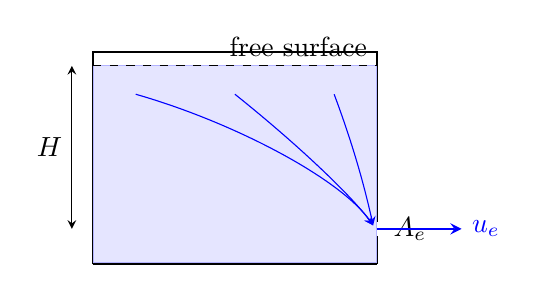
\begin{tikzpicture}[>=stealth, scale=0.9]
  % tank
  \draw[thick] (-2,0) -- (-2,3) -- (2,3) -- (2,0.6);
  \draw[thick] (2,0.4) -- (2,0);
  \draw[thick] (-2,0) -- (2,0);
  \draw[blue!30,fill=blue!10] (-2,0.02) rectangle (2,2.8);
  \draw[dashed] (-2,2.8) -- (2,2.8) node[above left] {free surface};
  \draw[<->] (-2.3,0.5) -- (-2.3,2.8) node[midway,left] {$H$};
  \node[right] at (2.1,0.5) {$A_e$};
  \draw[->,thick,blue] (2,0.5) -- (3.2,0.5) node[right] {$u_e$};
  % streamlines
  \draw[->,blue] (-1.4,2.4) .. controls (0,2.0) and (1.5,1.2) .. (1.95,0.55);
  \draw[->,blue] (0,2.4) .. controls (1,1.6) and (1.7,0.9) .. (1.95,0.55);
  \draw[->,blue] (1.4,2.4) .. controls (1.7,1.6) and (1.85,1.0) .. (1.95,0.55);
\end{tikzpicture}
\end{center}

%==============================================================
\section*{Question 3 --- Bifurcations and 2-D phase portrait}

\textbf{Problem.} Analyse $\dot x=rx-2x^{2}+x^{3}$: fixed points, stability, bifurcations $r_1,r_2$, normal forms. Then phase-portrait $\dot x=x^{2}-y-1$, $\dot y=(x-2)y$.

\subsection*{Fixed point $x^{*}=0$}

Set $\dot x=0$:
\[ x(r-2x+x^{2})=0. \]
$x=0$ is always a root. Stability from $f'(x)=r-4x+3x^{2}$:
\[ f'(0)=r. \]
Stable for $r<0$, unstable for $r>0$. Bifurcation at:
\[ \boxed{\;r_{1}=0.\;} \]

\subsection*{Other fixed points}

Other roots solve $x^{2}-2x+r=0$:
\[ x_{\pm}=\frac{2\pm\sqrt{4-4r}}{2}=1\pm\sqrt{1-r}. \]
Real for $r\le 1$. Use $x_\pm^{2}=2x_\pm-r$ in $f'(x)=r-4x+3x^{2}$:
\[ f'(x_\pm)=r-4x_\pm+3(2x_\pm-r). \]
Expand:
\[ f'(x_\pm)=r-4x_\pm+6x_\pm-3r. \]
Combine like terms:
\[ f'(x_\pm)=-2r+2x_\pm=2(x_\pm-r). \]
Substitute $x_\pm=1\pm\sqrt{1-r}$:
\[ f'(x_\pm)=2\bigl(1\pm\sqrt{1-r}-r\bigr)=2\bigl((1-r)\pm\sqrt{1-r}\bigr). \]
Factor $\sqrt{1-r}$:
\[ f'(x_\pm)=2\sqrt{1-r}\bigl(\sqrt{1-r}\pm 1\bigr). \]
For $0<r<1$: $\sqrt{1-r}>0$ and $\sqrt{1-r}-1<0$, so $f'(x_-)<0$ (stable); $\sqrt{1-r}+1>0$, so $f'(x_+)>0$ (unstable). Both vanish at $r=1$.

Second bifurcation at:
\[ \boxed{\;r_{2}=1.\;} \]
At $r=1$: $x_\pm=1$ collide (saddle-node). At $r=0$: $x_-=0$ collides with $x^{*}=0$ (transcritical; $x_+=2$ persists for all $r\le 1$).

\subsection*{Bifurcation diagram and normal forms}

\begin{center}
\begin{tikzpicture}[>=stealth, scale=1.0]
  \draw[->] (-2,0) -- (3.5,0) node[right] {$r$};
  \draw[->] (0,-1.0) -- (0,3.2) node[above] {$x$};
  \node[below left] at (0,0) {$0$};
  \node[below] at (1,0) {$r_2=1$};
  % x*=0 branch: stable r<0 (solid), unstable r>0 (dashed)
  \draw[thick] (-2,0) -- (0,0);
  \draw[thick,dashed] (0,0) -- (3.3,0);
  % x_-: from (0,0) to (1,1), stable (solid)
  \draw[thick,domain=0:1, samples=80, smooth, variable=\r] plot ({\r},{1-sqrt(1-\r)});
  % x_+: from (0,2) to (1,1), unstable (dashed)
  \draw[thick,dashed,domain=0:1, samples=80, smooth, variable=\r] plot ({\r},{1+sqrt(1-\r)});
  % markers at bifurcations
  \node[circle,fill,inner sep=1.2pt,label=below left:{$r_1$}] at (0,0) {};
  \node[circle,fill,inner sep=1.2pt,label=above right:{SN}] at (1,1) {};
  \node[left] at (0,2) {$x_+$};
  \node[right] at (1.05,0.3) {$x_-$};
  % flow arrows on x-axis
  \draw[->,gray] (-1.4,0.25) -- (-1.0,0.05);
  \draw[->,gray] (-1.4,-0.25) -- (-1.0,-0.05);
  \draw[->,gray] (2.3,0.05) -- (2.6,0.25);
\end{tikzpicture}
\end{center}

Solid = stable, dashed = unstable.

\textbf{Normal form at $r_1=0$:} drop the cubic $x^{3}$ (higher-order near $x=0$):
\[ \dot x\approx rx-2x^{2}. \]
Fixed points: $x=0$ and $x=r/2$ cross at $r=0$ and exchange stability:
\[ \boxed{\;\dot x=rx-2x^{2}\quad\text{(transcritical).}\;} \]

\textbf{Normal form at $r_2=1$:} let $r=1+\mu$, $x=1+y$ so $\dot x=\dot y$:
\[ \dot y=(1+\mu)(1+y)-2(1+y)^{2}+(1+y)^{3}. \]
Expand $(1+\mu)(1+y)$:
\[ (1+\mu)(1+y)=1+y+\mu+\mu y. \]
Expand $-2(1+y)^{2}$:
\[ -2(1+y)^{2}=-2-4y-2y^{2}. \]
Expand $(1+y)^{3}$:
\[ (1+y)^{3}=1+3y+3y^{2}+y^{3}. \]
Sum the three contributions:
\[ \dot y=(1-2+1)+(1-4+3)y+\mu+\mu y+(-2+3)y^{2}+y^{3}. \]
Collect (constants and linear in $y$ both vanish):
\[ \dot y=\mu+\mu y+y^{2}+y^{3}. \]
Drop higher orders $\mu y$, $y^{3}$ near $(\mu,y)=(0,0)$:
\[ \boxed{\;\dot y=\mu+y^{2}\quad\text{(saddle-node).}\;} \]

\subsection*{2-D phase portrait}

Set $\dot y=0$:
\[ (x-2)y=0\;\Rightarrow\;y=0\ \text{or}\ x=2. \]
On branch $y=0$, set $\dot x=0$:
\[ x^{2}-1=0\;\Rightarrow\;x=\pm 1. \]
On branch $x=2$, set $\dot x=0$:
\[ 4-y-1=0\;\Rightarrow\;y=3. \]
Fixed points: $(1,0),\,(-1,0),\,(2,3)$.

General Jacobian:
\[ J=\begin{pmatrix}\partial f_1/\partial x & \partial f_1/\partial y\\ \partial f_2/\partial x & \partial f_2/\partial y\end{pmatrix}=\begin{pmatrix}2x & -1\\ y & x-2\end{pmatrix}. \]

At $(1,0)$:
\[ J=\begin{pmatrix}2 & -1\\ 0 & -1\end{pmatrix},\quad \tau=1,\;\Delta=-2. \]
$\Delta<0$ implies saddle. Solve $\det(J-\lambda I)=(2-\lambda)(-1-\lambda)=0$:
\[ \lambda_1=2,\quad \lambda_2=-1. \]
Eigenvector for $\lambda_1=2$: $(J-2I)\vb v=0$ gives $-v_2=0$, so $v=(1,0)^{T}$ (unstable).
Eigenvector for $\lambda_2=-1$: $3v_1-v_2=0$, so $v=(1,3)^{T}$ (stable).

At $(-1,0)$:
\[ J=\begin{pmatrix}-2 & -1\\ 0 & -3\end{pmatrix},\quad \tau=-5,\;\Delta=6. \]
Compute discriminant:
\[ \tau^{2}-4\Delta=25-24=1>0. \]
With $\tau<0$, $\Delta>0$, $\tau^{2}>4\Delta$: stable node. Solve $\det(J-\lambda I)=(-2-\lambda)(-3-\lambda)=0$:
\[ \lambda_1=-2,\quad \lambda_2=-3. \]
Eigenvectors: $(J+2I)\vb v=0$ gives $v=(1,0)^{T}$; $(J+3I)\vb v=0$ gives $v_1-v_2=0$, so $v=(1,1)^{T}$.

At $(2,3)$:
\[ J=\begin{pmatrix}4 & -1\\ 3 & 0\end{pmatrix},\quad \tau=4,\;\Delta=3. \]
Compute discriminant:
\[ \tau^{2}-4\Delta=16-12=4>0. \]
With $\tau>0$, $\Delta>0$, $\tau^{2}>4\Delta$: unstable node. Solve $\lambda^{2}-4\lambda+3=0$:
\[ \lambda_1=1,\quad \lambda_2=3. \]
Eigenvector for $\lambda_1=1$: $3v_1-v_2=0$, so $v=(1,3)^{T}$.
Eigenvector for $\lambda_2=3$: $v_1-v_2=0$, so $v=(1,1)^{T}$.

Nullclines: $\dot x=0$ on parabola $y=x^{2}-1$; $\dot y=0$ on $y=0$ and $x=2$.

\begin{center}
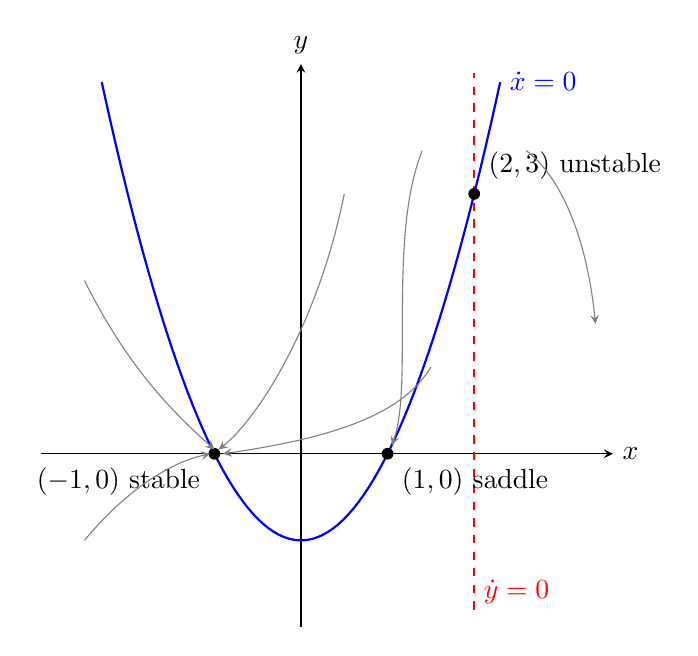
\begin{tikzpicture}[>=stealth, scale=1.1]
  \draw[->] (-3,0) -- (3.6,0) node[right] {$x$};
  \draw[->] (0,-2) -- (0,4.5) node[above] {$y$};
  % parabola y = x^2-1
  \draw[thick,blue,domain=-2.3:2.3,samples=80] plot (\x,{\x*\x-1});
  \node[blue,right] at (2.3,4.3) {$\dot x=0$};
  % x=2 line
  \draw[thick,red,dashed] (2,-1.8) -- (2,4.4);
  \node[red,right] at (2,-1.6) {$\dot y=0$};
  % fixed points with markers
  \node[circle,fill,inner sep=1.5pt,label=below right:{$(1,0)$ saddle}] at (1,0) {};
  \node[circle,fill,inner sep=1.5pt,label=below left:{$(-1,0)$ stable}] at (-1,0) {};
  \node[circle,fill,inner sep=1.5pt,label=above right:{$(2,3)$ unstable}] at (2,3) {};
  % schematic trajectories
  \draw[->,gray]   (-2.5,2)  .. controls (-2,1)  and (-1.5,0.5) .. (-1,0.05);
  \draw[->,gray]   (-2.5,-1) .. controls (-2,-0.4) and (-1.5,-0.1) .. (-1.05,0);
  \draw[->,gray]   (0.5,3)   .. controls (0.2,1.5) and (-0.5,0.4) .. (-0.95,0.05);
  \draw[->,gray]   (1.5,1)   .. controls (1.2,0.5) and (0.5,0.2) .. (-0.9,0.0);
  \draw[->,gray]   (2.6,3.5) .. controls (3.0,3.2) and (3.3,2.5) .. (3.4,1.5);
  \draw[->,gray]   (1.4,3.5) .. controls (1.0,2.5) and (1.3,0.8) .. (1.05,0.1);
\end{tikzpicture}
\end{center}

%==============================================================
\section*{Question 4 --- FJC, WLC and DNA}

\textbf{Problem.} Show $\langle r^{2}\rangle=Nb^{2}$ for FJC; derive WLC formula and limits; obtain Gaussian end-to-end distribution; show entropic spring $A=a+cr^{2}$ with $c$ in terms of $N,b,T$; high-force regime; numerical estimates for ds and ssDNA.

\subsection*{FJC: $\langle r^{2}\rangle=Nb^{2}$}

\begin{center}
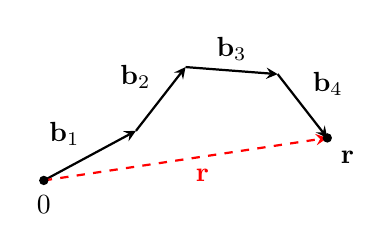
\begin{tikzpicture}[>=stealth, scale=0.9]
  \draw[->,thick] (0,0) -- (1.3,0.7) node[midway,above left] {$\vb b_1$};
  \draw[->,thick] (1.3,0.7) -- (2.0,1.6) node[midway,above left] {$\vb b_2$};
  \draw[->,thick] (2.0,1.6) -- (3.3,1.5) node[midway,above] {$\vb b_3$};
  \draw[->,thick] (3.3,1.5) -- (4.0,0.6) node[midway,above right] {$\vb b_4$};
  \draw[->,dashed,thick,red] (0,0) -- (4.0,0.6) node[midway,below right] {$\vb r$};
  \node[circle,fill,inner sep=1.2pt,label=below:{$0$}] at (0,0) {};
  \node[circle,fill,inner sep=1.2pt,label=below right:{$\vb r$}] at (4.0,0.6) {};
\end{tikzpicture}
\end{center}

End-to-end vector is the sum of $N$ segments of length $b$:
\[ \vb r=\sum_{i=1}^{N}\vb b_i,\qquad |\vb b_i|=b. \]
Square and split diagonal/off-diagonal:
\[ \vb r\cdot\vb r=\sum_{i=1}^{N}\vb b_i\cdot\vb b_i+\sum_{i\ne j}\vb b_i\cdot\vb b_j. \]
Evaluate diagonal terms ($\vb b_i\cdot\vb b_i=b^{2}$):
\[ \vb r\cdot\vb r=Nb^{2}+\sum_{i\ne j}\vb b_i\cdot\vb b_j. \]
Take ensemble average; non-interacting segments give $\langle\vb b_i\cdot\vb b_j\rangle=0$ for $i\ne j$:
\[ \boxed{\;\langle r^{2}\rangle=Nb^{2}.\;} \]

\subsection*{WLC: derivation and limits}

Continuous tangent:
\[ \vb r=\int_{0}^{L}\vb t(s)\,\de s,\qquad \langle\vb t(s)\cdot\vb t(s')\rangle=e^{-|s-s'|/P}. \]
Square and average:
\[ \langle r^{2}\rangle=\int_{0}^{L}\!\!\int_{0}^{L} e^{-|s-s'|/P}\,\de s\,\de s'. \]
Use symmetry $s'<s$, factor of $2$:
\[ \langle r^{2}\rangle=2\int_{0}^{L}\de s\int_{0}^{s}e^{-(s-s')/P}\de s'. \]
Substitute $u=s-s'$ in the inner integral:
\[ \int_{0}^{s}e^{-(s-s')/P}\de s'=\int_{0}^{s}e^{-u/P}\de u=P\bigl(1-e^{-s/P}\bigr). \]
Insert into outer integral:
\[ \langle r^{2}\rangle=2P\int_{0}^{L}\bigl(1-e^{-s/P}\bigr)\de s. \]
Evaluate the outer integral:
\[ \int_{0}^{L}\bigl(1-e^{-s/P}\bigr)\de s=L+P(e^{-L/P}-1). \]
Hence:
\[ \langle r^{2}\rangle=2P\bigl[L+P(e^{-L/P}-1)\bigr]. \]
\[ \boxed{\;\langle r^{2}\rangle=2P^{2}\!\left(e^{-L/P}-1+\frac{L}{P}\right).\;} \]

\textbf{Limit $L\gg P$:} $e^{-L/P}\to 0$:
\[ \langle r^{2}\rangle\to 2PL. \]
Identifies effective Kuhn length $b_K=2P$ and segment count $L/(2P)$: Gaussian-coil regime.

\textbf{Limit $L\ll P$:} expand $e^{-L/P}=1-L/P+L^{2}/(2P^{2})-\dots$:
\[ e^{-L/P}-1+L/P\approx L^{2}/(2P^{2}). \]
Multiply by $2P^{2}$:
\[ \langle r^{2}\rangle\to L^{2}. \]
Rigid-rod regime; chain too short to bend.

\subsection*{End-to-end distribution and width}

3-D Gaussian random walk: $x,y,z$ each diffuse independently in $N$ steps. For an isotropic random step, $\langle b_x^{2}\rangle=b^{2}/3$, so identify $2Dt\to Nb^{2}/3$ per axis:
\[ P_1(x_i,N)=\sqrt{\frac{3}{2\pi Nb^{2}}}\exp\!\left(-\frac{3x_i^{2}}{2Nb^{2}}\right). \]
Multiply three independent Gaussians $P(\vb r,N)=P_1(x)P_1(y)P_1(z)$:
\[ P(\vb r,N)=\left(\frac{3}{2\pi Nb^{2}}\right)^{3/2}\exp\!\left(-\frac{3(x^{2}+y^{2}+z^{2})}{2Nb^{2}}\right). \]
Use $r^{2}=x^{2}+y^{2}+z^{2}$:
\[ P(\vb r,N)=\left(\frac{3}{2\pi Nb^{2}}\right)^{3/2}\exp\!\left(-\frac{3r^{2}}{2Nb^{2}}\right). \]
\[ \boxed{\;P(\vb r,N)=\left(\frac{3}{2\pi Nb^{2}}\right)^{3/2}\exp\!\left(-\frac{3r^{2}}{2Nb^{2}}\right).\;} \]
Width along one axis $\sigma=\sqrt{Nb^{2}/3}$. Total $\langle r^{2}\rangle=3\sigma^{2}=Nb^{2}$, recovering the FJC result.

\begin{center}
\begin{tikzpicture}[>=stealth, scale=1.0]
  \begin{axis}[
    width=8.5cm, height=5cm,
    axis lines=left,
    xlabel={$r$}, ylabel={$4\pi r^{2}P(\vb r,N)$},
    xtick=\empty, ytick=\empty,
    xmin=0, xmax=4, ymin=0, ymax=1.0,
    domain=0:4, samples=200
  ]
    \addplot[thick, blue] {x*x*exp(-x*x/2)*0.6};
    \draw[dashed,gray] (axis cs:1.41,0) -- (axis cs:1.41,0.51);
    \node[below] at (axis cs:1.41,0) {$\sqrt{\langle r^{2}\rangle}$};
  \end{axis}
\end{tikzpicture}
\end{center}

\subsection*{Entropic spring}

Boltzmann entropy of conformations with end-to-end vector $\vb r$:
\[ S(\vb r)=k_B\ln\Omega(\vb r)=k_B\ln\bigl[V P(\vb r,N)\bigr]. \]
Insert Gaussian and split into $r$-independent / $r$-dependent parts:
\[ S(\vb r)=k_B\ln C-\frac{3k_B r^{2}}{2Nb^{2}}, \]
with $C$ collecting $r$-independent prefactors.
At fixed $T$, with internal energy $U$ independent of $\vb r$:
\[ A(\vb r)=U-TS(\vb r). \]
Substitute $S(\vb r)$:
\[ A(\vb r)=U-Tk_B\ln C+\frac{3k_B T}{2Nb^{2}}r^{2}. \]
Identify $a=U-Tk_B\ln C$, $c=3k_BT/(2Nb^{2})$:
\[ \boxed{\;A(\vb r)=a+cr^{2},\qquad c=\frac{3k_B T}{2Nb^{2}}.\;} \]
Quadratic in $r$ $\Rightarrow$ Hookean restoring force $\vb F=-\grad A=-2c\vb r$. Stiffness comes purely from entropy (more conformations available at small $|\vb r|$): an \emph{entropic spring}.

\subsection*{High-force limit}

Each segment couples to applied force $\vb F=F\hat{\vb z}$; one-segment partition function with $\de\Omega=\sin\theta\,\de\theta\,\de\varphi$:
\[ Z_1=\int_{0}^{2\pi}\!\!\de\varphi\int_{0}^{\pi}\!\!\frac{\sin\theta\,\de\theta}{4\pi}\,e^{\beta Fb\cos\theta}. \]
Evaluate (let $u=\cos\theta$):
\[ Z_1=\frac{1}{2}\int_{-1}^{1}e^{\beta Fb\,u}\,\de u=\frac{\sinh(\beta Fb)}{\beta Fb}. \]
Mean projection per segment via $\langle b_z\rangle=\partial\ln Z_1/\partial(\beta F)$:
\[ \langle b_z\rangle=b\,\mathcal{L}(\beta F b),\qquad \mathcal{L}(x)=\coth x-\tfrac{1}{x}. \]
Total extension over $N$ segments:
\[ z=N b\,\mathcal{L}(\beta F b). \]
High-force limit $\beta Fb\gg 1$: $\coth(\beta Fb)\to 1$:
\[ \mathcal{L}(\beta Fb)\to 1-\frac{1}{\beta Fb}=1-\frac{k_BT}{Fb}. \]
Hence:
\[ z\to Nb\!\left(1-\frac{k_BT}{Fb}\right). \]
Solve for $F$:
\[ 1-\frac{z}{Nb}=\frac{k_BT}{Fb}. \]
Rearrange:
\[ \boxed{\;F\simeq\frac{k_B T}{b}\,\frac{1}{1-z/(Nb)}.\;} \]
$F$ diverges as the chain approaches contour length $L=Nb$.

\subsection*{Bacterial DNA --- numerical estimates}

\textbf{Double-stranded:} contour length
\[ L=5\times 10^{6}\times 0.34\,\text{nm}=1.7\times 10^{6}\,\text{nm}=1.7\,\text{mm}. \]
Persistence length:
\[ P=150\times 0.34\,\text{nm}=51\,\text{nm}. \]
Use $L\gg P$ limit $\langle r^{2}\rangle\approx 2PL$:
\[ \langle r^{2}\rangle\approx 2(51)(1.7\times 10^{6})\,\text{nm}^{2}=1.73\times 10^{8}\,\text{nm}^{2}. \]
Take square root:
\[ \boxed{\;\sqrt{\langle r^{2}\rangle}_{\text{ds}}\approx 1.32\times 10^{4}\,\text{nm}=\SI{13.2}{\micro m}.\;} \]

\textbf{Single-stranded:} persistence length
\[ P_\text{ss}=5\times 0.34\,\text{nm}=1.7\,\text{nm}. \]
Apply $\langle r^{2}\rangle\approx 2P_\text{ss}L$:
\[ \langle r^{2}\rangle\approx 2(1.7)(1.7\times 10^{6})\,\text{nm}^{2}=5.78\times 10^{6}\,\text{nm}^{2}. \]
Take square root:
\[ \boxed{\;\sqrt{\langle r^{2}\rangle}_{\text{ss}}\approx 2.40\times 10^{3}\,\text{nm}=\SI{2.4}{\micro m}.\;} \]

\textbf{Probability ratio} $P(R{=}0)/P(R{=}50\,\mu\text{m})$. Use Gaussian with $Nb^{2}\to\langle r^{2}\rangle$:
\[ \frac{P(0)}{P(R)}=\exp\!\left(\frac{3R^{2}}{2\langle r^{2}\rangle}\right). \]

ds case: $R=50\,\mu\text{m}=5\times 10^{4}\,\text{nm}$, so $R^{2}=2.5\times 10^{9}\,\text{nm}^{2}$. Substitute $\langle r^{2}\rangle=1.73\times 10^{8}\,\text{nm}^{2}$:
\[ \frac{3R^{2}}{2\langle r^{2}\rangle}=\frac{3(2.5\times 10^{9})}{2(1.73\times 10^{8})}. \]
Evaluate:
\[ \frac{3R^{2}}{2\langle r^{2}\rangle}\approx 21.7. \]
Exponentiate:
\[ \boxed{\;P(0)/P(50\,\mu\text{m})_\text{ds}\approx e^{21.7}\approx 2.7\times 10^{9}.\;} \]

ss case: substitute $\langle r^{2}\rangle=5.78\times 10^{6}\,\text{nm}^{2}$:
\[ \frac{3R^{2}}{2\langle r^{2}\rangle}=\frac{3(2.5\times 10^{9})}{2(5.78\times 10^{6})}. \]
Evaluate:
\[ \frac{3R^{2}}{2\langle r^{2}\rangle}\approx 649. \]
Exponentiate:
\[ \boxed{\;P(0)/P(50\,\mu\text{m})_\text{ss}\approx e^{649}\sim 10^{282}.\;} \]

Comment: ssDNA is far more compact than dsDNA (smaller $P$, smaller $\langle r^{2}\rangle$); reaching $50\,\mu$m is astronomically improbable. Both ratios $\gg 1$: extended states are heavily entropically suppressed.

\textbf{Low-force regime.} Both behave as Hookean entropic springs with stiffness $k=3k_BT/\langle r^{2}\rangle$:
\[ F=\frac{3k_B T}{\langle r^{2}\rangle}\,z. \]
ssDNA has smaller $\langle r^{2}\rangle$ $\Rightarrow$ steeper slope (stiffer at low force). dsDNA has larger $\langle r^{2}\rangle$ $\Rightarrow$ softer at low force.

\begin{center}
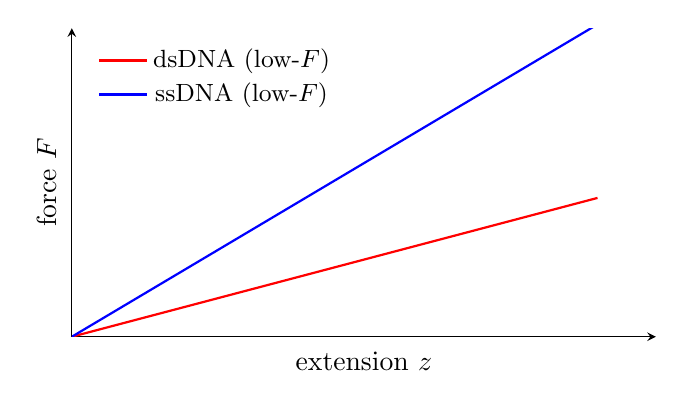
\begin{tikzpicture}[>=stealth, scale=1.0]
  \begin{axis}[
    width=9cm, height=5.5cm,
    axis lines=left,
    xlabel={extension $z$}, ylabel={force $F$},
    xtick=\empty, ytick=\empty,
    xmin=0, xmax=5, ymin=0, ymax=4,
    legend pos=north west,
    legend style={draw=none, font=\small}
  ]
    \addplot[thick, red,  domain=0:4.5, samples=80] {0.4*x};
    \addlegendentry{dsDNA (low-$F$)}
    \addplot[thick, blue, domain=0:4.5, samples=80] {0.9*x};
    \addlegendentry{ssDNA (low-$F$)}
  \end{axis}
\end{tikzpicture}
\end{center}

ssDNA (steeper) is entropically stiffer because its smaller persistence length yields a more compact equilibrium coil and thus a larger $3k_BT/\langle r^{2}\rangle$.

\end{document}
